
\documentclass[twocolumn]{revtex4-1}
\usepackage[latin9]{inputenc}
\usepackage{amsmath}
\setcounter{secnumdepth}{3}
\usepackage{upgreek}
\usepackage{amstext}
\usepackage{graphicx}  
\usepackage{changes}

\begin{document}
\title{Active Seismic Isolation with an Inertial Rotation Sensor}
\author{M.P. Ross, B. Lantz, E. Bonilla, A. Engl,  C.Gettings, E.A. Shaw,  and J.H. Gundlach}

\begin{abstract}

Active seismic isolation is indispensable for terrestrial gravitational wave observatories. Current systems utilize a variety of sensors and actuators to sense and control the motion of the isolated platform in all six degrees-of-freedom. To date, the inertial rotation sensing has been achieved utilizing the difference of displaced pairs of translational seismometers. We describe the implementation of a beam-balance based inertial rotation sensor on a dual-stage active isolation platform. This sensor achieves out-of-loop noise \added{XX} times lower than the existing sensors at \added{XX} Hz. With this sensor implemented within the table's control systems, the table's motion is decreased by \added{XX} compared to the seismometer-only implementation. 

\end{abstract}

\maketitle

\section{Introduction}

\section{Instrument}

\added{Sensor}

\added{ISI description}

\begin{figure}[!h]
\centering 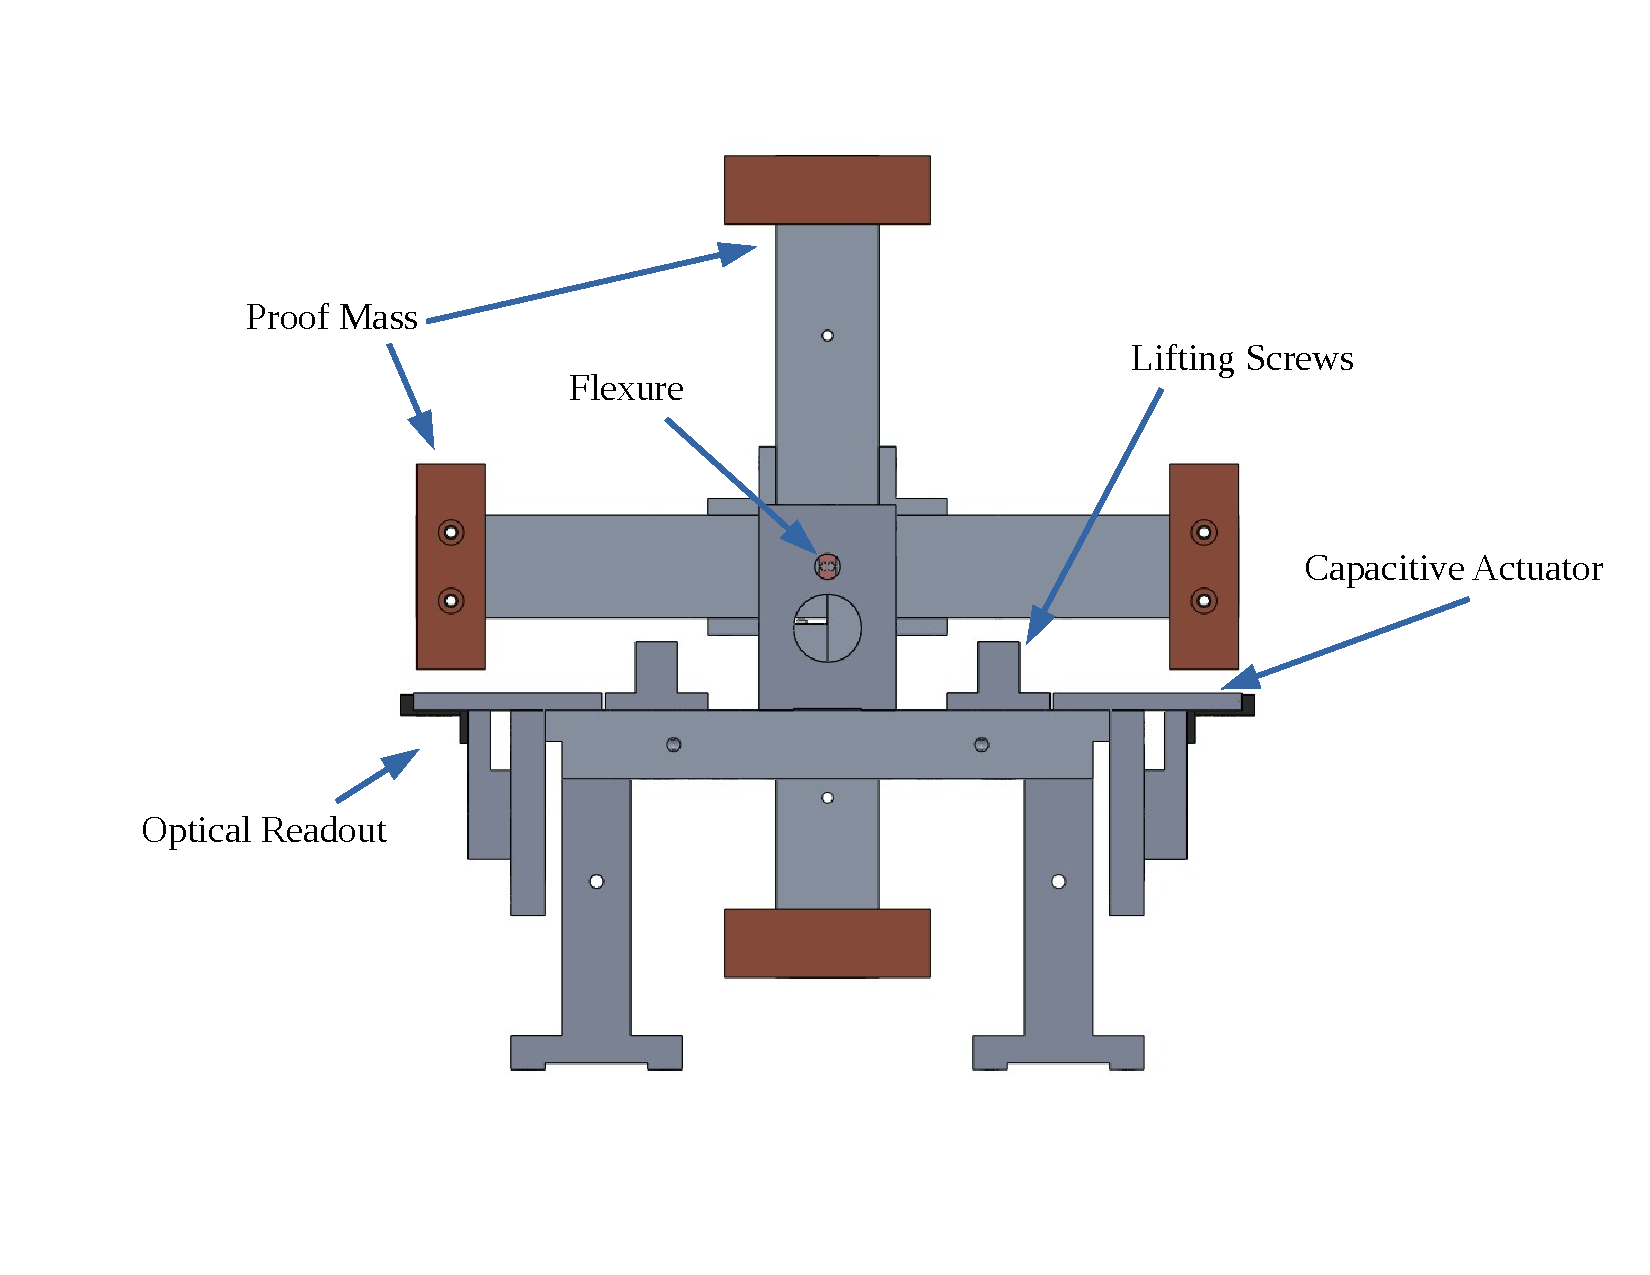
\includegraphics[width=0.5\textwidth]{cBRSFrontLabeled.pdf}
\caption{}
\label{apparatus} 
\end{figure}

\section{Out-of-Loop Measurements}

\added{Noise measurement}

\added{Transfer functions}

\begin{figure}[!h]
\centering 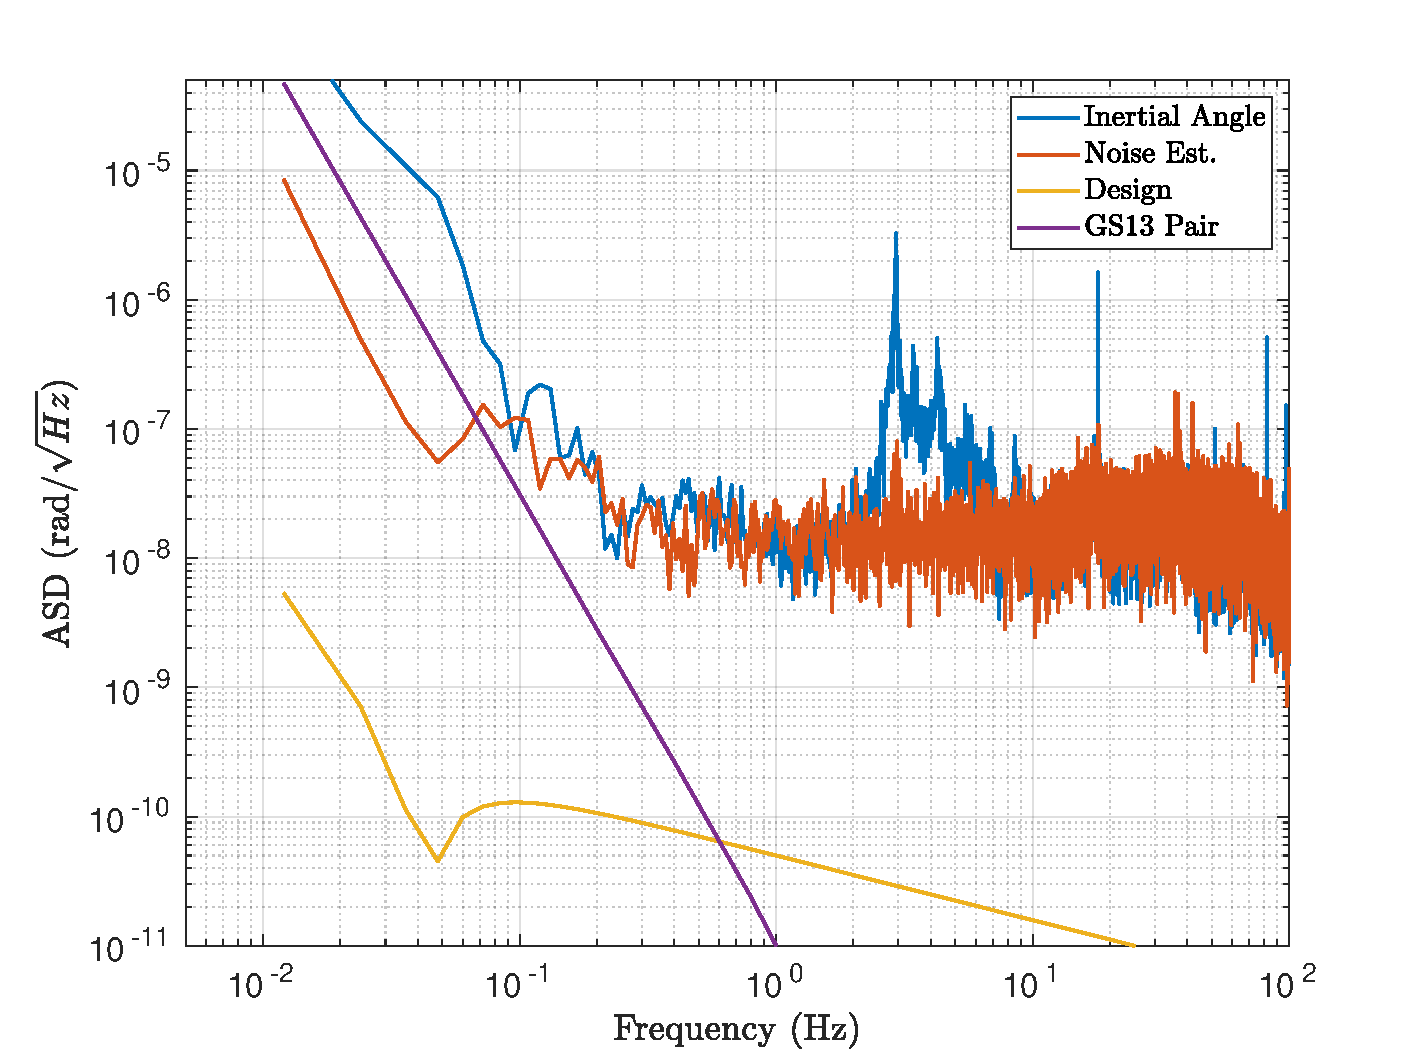
\includegraphics[width=0.5\textwidth]{cBRS_Stanford_InAir_TableLocked.pdf}
\caption{\added{REPLACE WITH TABLE CONTROLLED NOISE}}
\label{outloop} 
\end{figure}

\section{In-Loop Performance}

\added{Blends}

\added{Performance}

\begin{figure}[!h]
\centering 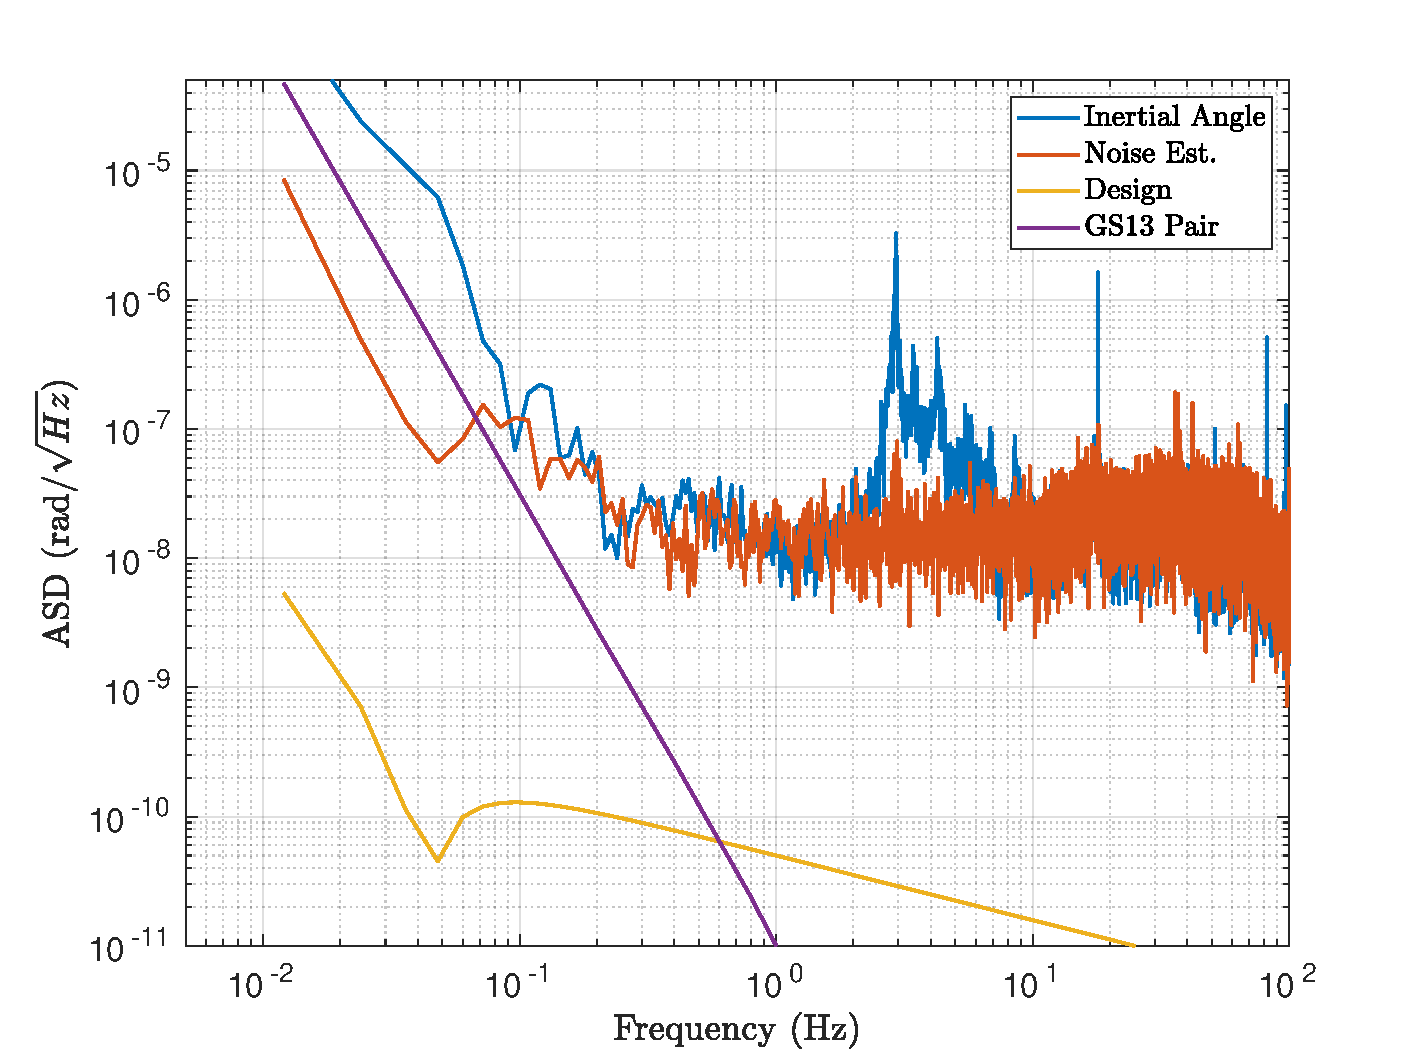
\includegraphics[width=0.5\textwidth]{cBRS_Stanford_InAir_TableLocked.pdf}
\caption{\added{REPLACE WITH IN LOOP PERFORMANCE. Compare to previous configuration}}
\label{inloop} 
\end{figure}

\section{Conclusion}

 \bibliographystyle{unsrtnat}
\bibliography{SuperconEP.bib}

\end{document}
